% cex-antidote.tex

\documentclass{standalone}
% newcommands.tex

\newcommand{\enq}{\texttt{enq}}
\newcommand{\deq}{\texttt{deq}}
\newcommand{\pput}{\texttt{PUT}}
\newcommand{\get}{\texttt{GET}}
\newcommand{\vs}{\texttt{vis}}
\newcommand{\so}{\texttt{so}}
\newcommand{\arb}{\texttt{ar}}
\newcommand{\rf}{\texttt{rf}}

% example
\newcommand{\po}[2]{\draw [->, thick] (#1) to node[above] {\Large{\so}} (#2);}
\newcommand{\pva}[2]{\draw [->, thick] (#1) to node[above] {$\Large{\so},\Large{\vs},\Large{\arb}$} (#2);}
\newcommand{\pbva}[2]{\draw [->, thick] (#1) to node[above] {$\Large{\so}$} node[below] {$\Large{\vs},\Large{\arb}$} (#2);}
\newcommand{\pv}[2]{\draw [->, thick] (#1) to node[above] {\Large{\so}} node[below] {\Large{\vs}} (#2);}
\newcommand{\evis}[2]{\draw [->, thick] (#1) to node[above, sloped, near end] {\Large{\vs}} (#2);}
\newcommand{\mvis}[2]{\draw [->, thick] (#1) to node[above, sloped] {\Large{\vs}} (#2);}
\newcommand{\ar}[2]{\draw [->, thick, allow upside down] (#1) to node[above, sloped] {\Large{\arb}} (#2);}
\newcommand{\va}[2]{\draw [->, thick, allow upside down] (#1) to node[above, sloped] {$\Large{\vs},\Large{\arb}$} (#2);}
\newcommand{\vab}[2]{\draw [->, thick, allow upside down] (#1) to node[below, sloped, near end] {$\Large{\vs},\Large{\arb}$} (#2);}
\newcommand{\vae}[2]{\draw [->, thick, allow upside down] (#1) to node[above, sloped, near end] {$\Large{\vs},\Large{\arb}$} (#2);}
\newcommand{\vas}[2]{\draw [->, thick, allow upside down] (#1) to node[sloped, near start, above] {$\Large{\vs},\Large{\arb}$} (#2);}

% serialization
\newcommand{\scc}[2]{\draw [->, very thick] (#1) to (#2);}
\newcommand{\rva}[2]{\draw [->, thick, allow upside down] (#1) to node[above, sloped] {$\Large{\rf},\Large{\vs},\Large{\arb}$} (#2);}
\newcommand{\rvb}[2]{\draw [->, thick, allow upside down] (#1) to node[below, sloped] {$\Large{\rf},\Large{\vs},\Large{\arb}$} (#2);}


\usepackage{tikz}
\usetikzlibrary{shapes, positioning, arrows.meta, decorations.pathmorphing}

\begin{document}
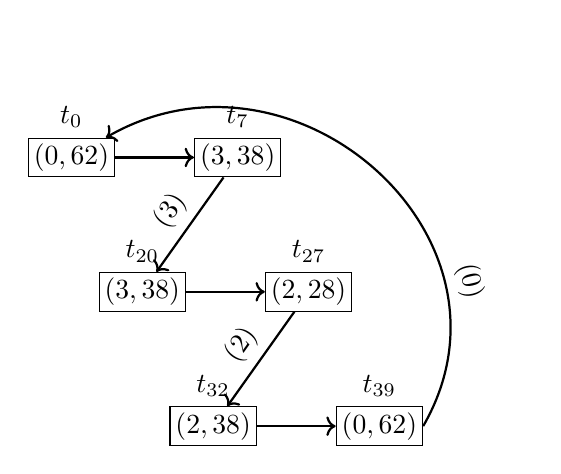
\begin{tikzpicture}[
  so/.style = {->, thick},
  wr/.style = {->, thick},
  co/.style = {->, thick},
  vo/.style = {->, thick},
  txn/.style = {draw, inner sep = 2pt}]
  \def\radius{5cm}

  \node[txn, label = above : $t_{0}$] (t0) {$\readevent(0, 62)$};
  \node[txn, label = above : $t_{7}$, right = of t0] (t7) {$\writeevent(3, 38)$};
  \node[txn, label = above : $t_{20}$, below left = 1.20cm and 0.10cm of t7] (t20) {$\readevent(3, 38)$};
  \node[txn, label = above : $t_{27}$, right = of t20] (t27) {$\writeevent(2, 28)$};
  \node[txn, label = above : $t_{32}$, below left = 1.20cm and 0.10cm of t27] (t32) {$\readevent(2, 38)$};
  \node[txn, label = above : $t_{39}$, right = of t32] (t39) {$\writeevent(0, 62)$};

  % \foreach \index/\label/\pos/\ops in {
  %     1/0/right/{\cdots \readevent(0, 62) \cdots},
  %     2/7/right/{\cdots \writeevent(3, 38) \cdots},
  %     3/20/left/{\cdots \readevent(3, 38) \cdots},
  %     4/27/left/{\cdots \writeevent(2, 28) \cdots},
  %     5/32/left/{\cdots \readevent(2, 28) \cdots},
  %     6/39/right/{\cdots \writeevent(0, 62) \cdots}} {
  %   \node[txn, label = \pos : $t_{\label}$]
  %     (t\label) at ({60 * (1- \index)}:\radius) {$\ops$};
  % }

  % t0-SO-t7
  \draw[so] (t0) to node[sloped, above]{$\SO$} (t7);
  % t7-WR-t20
  \draw[wr] (t7) to node[sloped, above]{$\WR(3)$} (t20);
  % t20-SO-t27
  \draw[so] (t20) to node[sloped, above]{$\SO$} (t27);
  % t27-WR-t32
  \draw[wr] (t27) to node[sloped, above]{$\WR(2)$} (t32);
  % t32-SO-t39
  \draw[so] (t32) to node[sloped, above]{$\SO$} (t39);
  % t39-WR-t0
  \draw[wr, out = 60, in = 30, looseness = 1.3] (t39.east)
    to node[sloped, above, near start]{$\WR(0)$} (t0);
\end{tikzpicture}
\end{document}